\documentclass[]{article}
\usepackage{lmodern}
\usepackage{amssymb,amsmath}
\usepackage{ifxetex,ifluatex}
\usepackage{fixltx2e} % provides \textsubscript
\ifnum 0\ifxetex 1\fi\ifluatex 1\fi=0 % if pdftex
  \usepackage[T1]{fontenc}
  \usepackage[utf8]{inputenc}
\else % if luatex or xelatex
  \ifxetex
    \usepackage{mathspec}
  \else
    \usepackage{fontspec}
  \fi
  \defaultfontfeatures{Ligatures=TeX,Scale=MatchLowercase}
\fi
% use upquote if available, for straight quotes in verbatim environments
\IfFileExists{upquote.sty}{\usepackage{upquote}}{}
% use microtype if available
\IfFileExists{microtype.sty}{%
\usepackage{microtype}
\UseMicrotypeSet[protrusion]{basicmath} % disable protrusion for tt fonts
}{}
\usepackage{hyperref}
\hypersetup{unicode=true,
            pdftitle={Arranging logger data from HoboLink and importing them to the database},
            pdfauthor={Jens Åström},
            pdfborder={0 0 0},
            breaklinks=true}
\urlstyle{same}  % don't use monospace font for urls
\usepackage{color}
\usepackage{fancyvrb}
\newcommand{\VerbBar}{|}
\newcommand{\VERB}{\Verb[commandchars=\\\{\}]}
\DefineVerbatimEnvironment{Highlighting}{Verbatim}{commandchars=\\\{\}}
% Add ',fontsize=\small' for more characters per line
\usepackage{framed}
\definecolor{shadecolor}{RGB}{248,248,248}
\newenvironment{Shaded}{\begin{snugshade}}{\end{snugshade}}
\newcommand{\AlertTok}[1]{\textcolor[rgb]{0.94,0.16,0.16}{#1}}
\newcommand{\AnnotationTok}[1]{\textcolor[rgb]{0.56,0.35,0.01}{\textbf{\textit{#1}}}}
\newcommand{\AttributeTok}[1]{\textcolor[rgb]{0.77,0.63,0.00}{#1}}
\newcommand{\BaseNTok}[1]{\textcolor[rgb]{0.00,0.00,0.81}{#1}}
\newcommand{\BuiltInTok}[1]{#1}
\newcommand{\CharTok}[1]{\textcolor[rgb]{0.31,0.60,0.02}{#1}}
\newcommand{\CommentTok}[1]{\textcolor[rgb]{0.56,0.35,0.01}{\textit{#1}}}
\newcommand{\CommentVarTok}[1]{\textcolor[rgb]{0.56,0.35,0.01}{\textbf{\textit{#1}}}}
\newcommand{\ConstantTok}[1]{\textcolor[rgb]{0.00,0.00,0.00}{#1}}
\newcommand{\ControlFlowTok}[1]{\textcolor[rgb]{0.13,0.29,0.53}{\textbf{#1}}}
\newcommand{\DataTypeTok}[1]{\textcolor[rgb]{0.13,0.29,0.53}{#1}}
\newcommand{\DecValTok}[1]{\textcolor[rgb]{0.00,0.00,0.81}{#1}}
\newcommand{\DocumentationTok}[1]{\textcolor[rgb]{0.56,0.35,0.01}{\textbf{\textit{#1}}}}
\newcommand{\ErrorTok}[1]{\textcolor[rgb]{0.64,0.00,0.00}{\textbf{#1}}}
\newcommand{\ExtensionTok}[1]{#1}
\newcommand{\FloatTok}[1]{\textcolor[rgb]{0.00,0.00,0.81}{#1}}
\newcommand{\FunctionTok}[1]{\textcolor[rgb]{0.00,0.00,0.00}{#1}}
\newcommand{\ImportTok}[1]{#1}
\newcommand{\InformationTok}[1]{\textcolor[rgb]{0.56,0.35,0.01}{\textbf{\textit{#1}}}}
\newcommand{\KeywordTok}[1]{\textcolor[rgb]{0.13,0.29,0.53}{\textbf{#1}}}
\newcommand{\NormalTok}[1]{#1}
\newcommand{\OperatorTok}[1]{\textcolor[rgb]{0.81,0.36,0.00}{\textbf{#1}}}
\newcommand{\OtherTok}[1]{\textcolor[rgb]{0.56,0.35,0.01}{#1}}
\newcommand{\PreprocessorTok}[1]{\textcolor[rgb]{0.56,0.35,0.01}{\textit{#1}}}
\newcommand{\RegionMarkerTok}[1]{#1}
\newcommand{\SpecialCharTok}[1]{\textcolor[rgb]{0.00,0.00,0.00}{#1}}
\newcommand{\SpecialStringTok}[1]{\textcolor[rgb]{0.31,0.60,0.02}{#1}}
\newcommand{\StringTok}[1]{\textcolor[rgb]{0.31,0.60,0.02}{#1}}
\newcommand{\VariableTok}[1]{\textcolor[rgb]{0.00,0.00,0.00}{#1}}
\newcommand{\VerbatimStringTok}[1]{\textcolor[rgb]{0.31,0.60,0.02}{#1}}
\newcommand{\WarningTok}[1]{\textcolor[rgb]{0.56,0.35,0.01}{\textbf{\textit{#1}}}}
\usepackage{graphicx,grffile}
\makeatletter
\def\maxwidth{\ifdim\Gin@nat@width>\linewidth\linewidth\else\Gin@nat@width\fi}
\def\maxheight{\ifdim\Gin@nat@height>\textheight\textheight\else\Gin@nat@height\fi}
\makeatother
% Scale images if necessary, so that they will not overflow the page
% margins by default, and it is still possible to overwrite the defaults
% using explicit options in \includegraphics[width, height, ...]{}
\setkeys{Gin}{width=\maxwidth,height=\maxheight,keepaspectratio}
\IfFileExists{parskip.sty}{%
\usepackage{parskip}
}{% else
\setlength{\parindent}{0pt}
\setlength{\parskip}{6pt plus 2pt minus 1pt}
}
\setlength{\emergencystretch}{3em}  % prevent overfull lines
\providecommand{\tightlist}{%
  \setlength{\itemsep}{0pt}\setlength{\parskip}{0pt}}
\setcounter{secnumdepth}{0}
% Redefines (sub)paragraphs to behave more like sections
\ifx\paragraph\undefined\else
\let\oldparagraph\paragraph
\renewcommand{\paragraph}[1]{\oldparagraph{#1}\mbox{}}
\fi
\ifx\subparagraph\undefined\else
\let\oldsubparagraph\subparagraph
\renewcommand{\subparagraph}[1]{\oldsubparagraph{#1}\mbox{}}
\fi

%%% Use protect on footnotes to avoid problems with footnotes in titles
\let\rmarkdownfootnote\footnote%
\def\footnote{\protect\rmarkdownfootnote}

%%% Change title format to be more compact
\usepackage{titling}

% Create subtitle command for use in maketitle
\newcommand{\subtitle}[1]{
  \posttitle{
    \begin{center}\large#1\end{center}
    }
}

\setlength{\droptitle}{-2em}
  \title{Arranging logger data from HoboLink and importing them to the database}
  \pretitle{\vspace{\droptitle}\centering\huge}
  \posttitle{\par}
  \author{Jens Åström}
  \preauthor{\centering\large\emph}
  \postauthor{\par}
  \predate{\centering\large\emph}
  \postdate{\par}
  \date{28 October, 2020}


%\linespread{1.3}


% You know, for landscape
\usepackage{lscape}
\usepackage{pdfpages}


% pandoc does not parse latex env - https://groups.google.com/forum/?fromgroups=#!topic/pandoc-discuss/oZETB5Ii1Cw
\newcommand{\blandscape}{\begin{landscape}}
\newcommand{\elandscape}{\end{landscape}}

% Make new page before each section
%\let\stdsection\section
%\renewcommand\section{\newpage\stdsection}

% Highlight inline `code`
\usepackage{soul}
\usepackage{xcolor}

\definecolor{Light}{gray}{.97}
\sethlcolor{Light}

\let\OldTexttt\texttt
\renewcommand{\texttt}[1]{\OldTexttt{\hl{#1}}}


\clubpenalty=10000      %kara za sierotki
\widowpenalty=10000  % nie pozostawiaj wdów
\brokenpenalty=10000    % nie dziel wyrazów miêdzy stronami
\exhyphenpenalty=999999   % nie dziel s³ów z myœlnikiem
\righthyphenmin=3     % dziel minimum 3 litery

\renewcommand{\topfraction}{0.95}
\renewcommand{\bottomfraction}{0.95}
\renewcommand{\textfraction}{0.05}
\renewcommand{\floatpagefraction}{0.35}

\begin{document}
\maketitle

{
\setcounter{tocdepth}{2}
\tableofcontents
}
\hypertarget{intro}{%
\section{Intro}\label{intro}}

The data exports for the temperature and humidity MX loggers from Hobo
needs a bit of data wrangling before it can be used. The different data
streams from each logger all get a separate column. Here we develop a
script to turn this into a more usable long format. We also make tables
in a database and upload the data there.

\hypertarget{read-in-data}{%
\section{Read in data}\label{read-in-data}}

We have an export file from Hobolink.com with many loggers as a csv
file. We also have some individual csv files that failed to upload to
the Hobo site, that we'll handle later on.

\begin{Shaded}
\begin{Highlighting}[]
\NormalTok{inputFile <-}\StringTok{ "../rawData/Insektoverv_k_2020_2020_10_27_12_07_50_UTC_1.csv"}

\NormalTok{rawDat <-}\StringTok{ }\KeywordTok{read_csv}\NormalTok{(inputFile,}\DataTypeTok{col_types =} \KeywordTok{cols}\NormalTok{(}\DataTypeTok{.default =} \StringTok{"c"}\NormalTok{))}

\NormalTok{dat <-}\StringTok{ }\NormalTok{rawDat }\OperatorTok\StringTok{  }
\StringTok{  }\KeywordTok{select}\NormalTok{(}\OperatorTok{-}\StringTok{"Line#"}\NormalTok{) }\OperatorTok\StringTok{ }
\StringTok{  }\KeywordTok{mutate}\NormalTok{(}\DataTypeTok{date =} \KeywordTok{as.POSIXct}\NormalTok{(Date, }\DataTypeTok{format =} \StringTok{"%m/%d/%y %H:%M:%S"}\NormalTok{)) }\OperatorTok\StringTok{ }
\StringTok{  }\KeywordTok{mutate_if}\NormalTok{(is_character, as.double) }\OperatorTok\StringTok{ }
\StringTok{  }\KeywordTok{select}\NormalTok{(}\OperatorTok{-}\NormalTok{Date)}
\end{Highlighting}
\end{Shaded}

\begin{verbatim}
## Warning in mask$eval_all_mutate(dots[[i]]): NAs introduced by coercion
\end{verbatim}

\begin{Shaded}
\begin{Highlighting}[]
\NormalTok{dat}
\end{Highlighting}
\end{Shaded}

\begin{verbatim}
## # A tibble: 132,522 x 61
##    `Temperature (M~ `RH (MX-RH-2 20~ `Dew Point (MX-~ `Temperature (M~
##               <dbl>            <dbl>            <dbl>            <dbl>
##  1             20.8             29.6             2.4              NA  
##  2             22.2             31.5             4.48             NA  
##  3             NA               NA              NA                22.3
##  4             24.9             25.4             3.77             NA  
##  5             NA               NA              NA                24.7
##  6             26.2             23.3             3.62             NA  
##  7             NA               NA              NA                25.5
##  8             26.6             23.0             3.78             NA  
##  9             NA               NA              NA                26.1
## 10             27.2             22.7             4.13             NA  
## # ... with 132,512 more rows, and 57 more variables: `RH (MX-RH-2
## #   20835814:20835814-2), %, 20835814` <dbl>, `Dew Point (MX-TEMP-2
## #   20835814:20835814-4), *C, 20835814` <dbl>, `Temperature (MX-TEMP-2
## #   20843239:20843239-1), *C, 20843239` <dbl>, `RH (MX-RH-2
## #   20843239:20843239-2), %, 20843239` <dbl>, `Dew Point (MX-TEMP-2
## #   20843239:20843239-4), *C, 20843239` <dbl>, `Temperature (MX-TEMP-2
## #   20843238:20843238-1), *C, 20843238` <dbl>, `RH (MX-RH-2
## #   20843238:20843238-2), %, 20843238` <dbl>, `Dew Point (MX-TEMP-2
## #   20843238:20843238-4), *C, 20843238` <dbl>, `Temperature (MX-TEMP-2
## #   20843235:20843235-1), *C, 20843235` <dbl>, `RH (MX-RH-2
## #   20843235:20843235-2), %, 20843235` <dbl>, `Dew Point (MX-TEMP-2
## #   20843235:20843235-4), *C, 20843235` <dbl>, `Temperature (MX-TEMP-2
## #   20843233:20843233-1), *C, 20843233` <dbl>, `RH (MX-RH-2
## #   20843233:20843233-2), %, 20843233` <dbl>, `Dew Point (MX-TEMP-2
## #   20843233:20843233-4), *C, 20843233` <dbl>, `Temperature (MX-TEMP-2
## #   20843231:20843231-1), *C, 20843231` <dbl>, `RH (MX-RH-2
## #   20843231:20843231-2), %, 20843231` <dbl>, `Dew Point (MX-TEMP-2
## #   20843231:20843231-4), *C, 20843231` <dbl>, `Temperature (MX-TEMP-2
## #   20843230:20843230-1), *C, 20843230` <dbl>, `RH (MX-RH-2
## #   20843230:20843230-2), %, 20843230` <dbl>, `Dew Point (MX-TEMP-2
## #   20843230:20843230-4), *C, 20843230` <dbl>, `Temperature (MX-TEMP-2
## #   20843229:20843229-1), *C, 20843229` <dbl>, `RH (MX-RH-2
## #   20843229:20843229-2), %, 20843229` <dbl>, `Dew Point (MX-TEMP-2
## #   20843229:20843229-4), *C, 20843229` <dbl>, `Temperature (MX-TEMP-2
## #   20843228:20843228-1), *C, 20843228` <dbl>, `RH (MX-RH-2
## #   20843228:20843228-2), %, 20843228` <dbl>, `Dew Point (MX-TEMP-2
## #   20843228:20843228-4), *C, 20843228` <dbl>, `Temperature (MX-TEMP-2
## #   20835825:20835825-1), *C, 20835825` <dbl>, `RH (MX-RH-2
## #   20835825:20835825-2), %, 20835825` <dbl>, `Dew Point (MX-TEMP-2
## #   20835825:20835825-4), *C, 20835825` <dbl>, `Temperature (MX-TEMP-2
## #   20835824:20835824-1), *C, 20835824` <dbl>, `RH (MX-RH-2
## #   20835824:20835824-2), %, 20835824` <dbl>, `Dew Point (MX-TEMP-2
## #   20835824:20835824-4), *C, 20835824` <dbl>, `Temperature (MX-TEMP-2
## #   20835823:20835823-1), *C, 20835823` <dbl>, `RH (MX-RH-2
## #   20835823:20835823-2), %, 20835823` <dbl>, `Dew Point (MX-TEMP-2
## #   20835823:20835823-4), *C, 20835823` <dbl>, `Temperature (MX-TEMP-2
## #   20835822:20835822-1), *C, 20835822` <dbl>, `RH (MX-RH-2
## #   20835822:20835822-2), %, 20835822` <dbl>, `Dew Point (MX-TEMP-2
## #   20835822:20835822-4), *C, 20835822` <dbl>, `Temperature (MX-TEMP-2
## #   20835821:20835821-1), *C, 20835821` <dbl>, `RH (MX-RH-2
## #   20835821:20835821-2), %, 20835821` <dbl>, `Dew Point (MX-TEMP-2
## #   20835821:20835821-4), *C, 20835821` <dbl>, `Temperature (MX-TEMP-2
## #   20835820:20835820-1), *C, 20835820` <dbl>, `RH (MX-RH-2
## #   20835820:20835820-2), %, 20835820` <dbl>, `Dew Point (MX-TEMP-2
## #   20835820:20835820-4), *C, 20835820` <dbl>, `Temperature (MX-TEMP-2
## #   20835819:20835819-1), *C, 20835819` <dbl>, `RH (MX-RH-2
## #   20835819:20835819-2), %, 20835819` <dbl>, `Dew Point (MX-TEMP-2
## #   20835819:20835819-4), *C, 20835819` <dbl>, `Temperature (MX-TEMP-2
## #   20835818:20835818-1), *C, 20835818` <dbl>, `RH (MX-RH-2
## #   20835818:20835818-2), %, 20835818` <dbl>, `Dew Point (MX-TEMP-2
## #   20835818:20835818-4), *C, 20835818` <dbl>, `Temperature (MX-TEMP-2
## #   20835817:20835817-1), *C, 20835817` <dbl>, `RH (MX-RH-2
## #   20835817:20835817-2), %, 20835817` <dbl>, `Dew Point (MX-TEMP-2
## #   20835817:20835817-4), *C, 20835817` <dbl>, `Temperature (MX-TEMP-2
## #   20835815:20835815-1), *C, 20835815` <dbl>, `RH (MX-RH-2
## #   20835815:20835815-2), %, 20835815` <dbl>, `Dew Point (MX-TEMP-2
## #   20835815:20835815-4), *C, 20835815` <dbl>, date <dttm>
\end{verbatim}

That's quite the number of columns\ldots{}

We have to pivot this data set to a longer format. We also get rid of
the rows with no data.

\begin{Shaded}
\begin{Highlighting}[]
\NormalTok{temp <-}\StringTok{ }\NormalTok{dat }\OperatorTok\StringTok{ }
\StringTok{  }\KeywordTok{pivot_longer}\NormalTok{(}\DataTypeTok{cols =} \KeywordTok{starts_with}\NormalTok{(}\StringTok{"Temperature"}\NormalTok{),}
               \DataTypeTok{names_to =} \StringTok{"logger_id"}\NormalTok{,}
               \DataTypeTok{values_to =} \StringTok{"temperature"}\NormalTok{) }\OperatorTok\StringTok{ }
\StringTok{  }\KeywordTok{select}\NormalTok{(date,}
\NormalTok{         logger_id,}
\NormalTok{         temperature) }\OperatorTok\StringTok{ }
\StringTok{  }\KeywordTok{filter}\NormalTok{(}\OperatorTok{!}\KeywordTok{is.na}\NormalTok{(temperature))}

\NormalTok{rh <-}\StringTok{ }\NormalTok{dat }\OperatorTok\StringTok{ }
\StringTok{  }\KeywordTok{pivot_longer}\NormalTok{(}\DataTypeTok{cols =} \KeywordTok{starts_with}\NormalTok{(}\StringTok{"RH"}\NormalTok{),}
               \DataTypeTok{names_to =} \StringTok{"logger_id"}\NormalTok{,}
               \DataTypeTok{values_to =} \StringTok{"rh"}\NormalTok{) }\OperatorTok\StringTok{ }
\StringTok{  }\KeywordTok{select}\NormalTok{(date,}
\NormalTok{         logger_id,}
\NormalTok{         rh)}\OperatorTok\StringTok{ }
\StringTok{  }\KeywordTok{filter}\NormalTok{(}\OperatorTok{!}\KeywordTok{is.na}\NormalTok{(rh))}

\NormalTok{dew  <-}\StringTok{ }\NormalTok{dat }\OperatorTok\StringTok{ }
\StringTok{  }\KeywordTok{pivot_longer}\NormalTok{(}\DataTypeTok{cols =} \KeywordTok{starts_with}\NormalTok{(}\StringTok{"Dew"}\NormalTok{),}
               \DataTypeTok{names_to =} \StringTok{"logger_id"}\NormalTok{,}
               \DataTypeTok{values_to =} \StringTok{"dew"}\NormalTok{) }\OperatorTok\StringTok{ }
\StringTok{  }\KeywordTok{select}\NormalTok{(date,}
\NormalTok{         logger_id,}
\NormalTok{         dew) }\OperatorTok\StringTok{ }
\StringTok{  }\KeywordTok{filter}\NormalTok{(}\OperatorTok{!}\KeywordTok{is.na}\NormalTok{(dew))}
\end{Highlighting}
\end{Shaded}

The data now looks like this

\begin{Shaded}
\begin{Highlighting}[]
\NormalTok{temp}
\end{Highlighting}
\end{Shaded}

\begin{verbatim}
## # A tibble: 132,522 x 3
##    date                logger_id                                     temperature
##    <dttm>              <chr>                                               <dbl>
##  1 2020-05-14 08:21:51 Temperature (MX-TEMP-2 20843236:20843236-1),~        20.8
##  2 2020-05-14 08:41:51 Temperature (MX-TEMP-2 20843236:20843236-1),~        22.2
##  3 2020-05-14 08:54:29 Temperature (MX-TEMP-2 20835814:20835814-1),~        22.3
##  4 2020-05-14 09:01:51 Temperature (MX-TEMP-2 20843236:20843236-1),~        24.9
##  5 2020-05-14 09:14:29 Temperature (MX-TEMP-2 20835814:20835814-1),~        24.7
##  6 2020-05-14 09:21:51 Temperature (MX-TEMP-2 20843236:20843236-1),~        26.2
##  7 2020-05-14 09:34:29 Temperature (MX-TEMP-2 20835814:20835814-1),~        25.5
##  8 2020-05-14 09:41:51 Temperature (MX-TEMP-2 20843236:20843236-1),~        26.6
##  9 2020-05-14 09:54:29 Temperature (MX-TEMP-2 20835814:20835814-1),~        26.1
## 10 2020-05-14 10:01:51 Temperature (MX-TEMP-2 20843236:20843236-1),~        27.2
## # ... with 132,512 more rows
\end{verbatim}

Time to strip the logger names and merge the tables

\begin{Shaded}
\begin{Highlighting}[]
\NormalTok{temp <-}\StringTok{ }\NormalTok{temp }\OperatorTok\StringTok{ }
\StringTok{  }\KeywordTok{mutate}\NormalTok{(}\DataTypeTok{logger_id =} \KeywordTok{str_extract}\NormalTok{(logger_id,}
                              \StringTok{"[^, ]+$"}\NormalTok{))}

\NormalTok{rh <-}\StringTok{ }\NormalTok{rh }\OperatorTok\StringTok{ }
\StringTok{  }\KeywordTok{mutate}\NormalTok{(}\DataTypeTok{logger_id =} \KeywordTok{str_extract}\NormalTok{(logger_id,}
                              \StringTok{"[^, ]+$"}\NormalTok{))}
\NormalTok{dew <-}\StringTok{ }\NormalTok{dew }\OperatorTok\StringTok{ }
\StringTok{  }\KeywordTok{mutate}\NormalTok{(}\DataTypeTok{logger_id =} \KeywordTok{str_extract}\NormalTok{(logger_id,}
                              \StringTok{"[^, ]+$"}\NormalTok{))}
\end{Highlighting}
\end{Shaded}

Check to see that the dates are the same for the datasets

\begin{Shaded}
\begin{Highlighting}[]
\KeywordTok{all}\NormalTok{(}\KeywordTok{all}\NormalTok{(temp}\OperatorTok{$}\NormalTok{date }\OperatorTok{==}\StringTok{ }\NormalTok{rh}\OperatorTok{$}\NormalTok{date),}
\KeywordTok{all}\NormalTok{(rh}\OperatorTok{$}\NormalTok{date }\OperatorTok{==}\StringTok{ }\NormalTok{dew}\OperatorTok{$}\NormalTok{date))}
\end{Highlighting}
\end{Shaded}

\begin{verbatim}
## [1] TRUE
\end{verbatim}

\begin{Shaded}
\begin{Highlighting}[]
\NormalTok{combDat <-}\StringTok{ }\NormalTok{temp }\OperatorTok\StringTok{ }
\StringTok{  }\KeywordTok{full_join}\NormalTok{(rh,}
             \DataTypeTok{by =} \KeywordTok{c}\NormalTok{(}\StringTok{"date"}\NormalTok{ =}\StringTok{ "date"}\NormalTok{,}
                    \StringTok{"logger_id"}\NormalTok{ =}\StringTok{ "logger_id"}\NormalTok{)) }\OperatorTok\StringTok{ }
\StringTok{  }\KeywordTok{full_join}\NormalTok{(dew,}
            \DataTypeTok{by =} \KeywordTok{c}\NormalTok{(}\StringTok{"date"}\NormalTok{ =}\StringTok{ "date"}\NormalTok{,}
                    \StringTok{"logger_id"}\NormalTok{ =}\StringTok{ "logger_id"}\NormalTok{)) }\OperatorTok\StringTok{ }
\StringTok{  }\KeywordTok{arrange}\NormalTok{(logger_id,}
\NormalTok{          date) }\OperatorTok\StringTok{ }
\StringTok{    }\KeywordTok{mutate}\NormalTok{(}\DataTypeTok{logger_type =} \StringTok{"MX2301A"}\NormalTok{) }\OperatorTok\StringTok{ }
\StringTok{    }\KeywordTok{select}\NormalTok{(date, }
\NormalTok{           logger_type,}
\NormalTok{           logger_id,}
\NormalTok{           temperature,}
\NormalTok{           rh,}
\NormalTok{           dew)}
\end{Highlighting}
\end{Shaded}

\begin{Shaded}
\begin{Highlighting}[]
\NormalTok{combDat}
\end{Highlighting}
\end{Shaded}

\begin{verbatim}
## # A tibble: 132,522 x 6
##    date                logger_type logger_id temperature    rh   dew
##    <dttm>              <chr>       <chr>           <dbl> <dbl> <dbl>
##  1 2020-05-14 08:54:29 MX2301A     20835814        22.3   28.2  3.05
##  2 2020-05-14 09:14:29 MX2301A     20835814        24.7   25.6  3.69
##  3 2020-05-14 09:34:29 MX2301A     20835814        25.5   24.4  3.72
##  4 2020-05-14 09:54:29 MX2301A     20835814        26.1   24.0  3.95
##  5 2020-05-14 10:14:29 MX2301A     20835814        26.5   23.2  3.83
##  6 2020-05-14 10:34:29 MX2301A     20835814        26.5   23.3  3.91
##  7 2020-05-14 10:54:29 MX2301A     20835814        20.6   19.5 -3.47
##  8 2020-05-14 11:14:29 MX2301A     20835814         5.32  47.9 -4.83
##  9 2020-05-14 11:34:29 MX2301A     20835814         4.53  53.3 -4.13
## 10 2020-05-14 14:39:05 MX2301A     20835814         1.88  79.3 -1.32
## # ... with 132,512 more rows
\end{verbatim}

\hypertarget{package-this-into-a-function}{%
\section{Package this into a
function}\label{package-this-into-a-function}}

\begin{Shaded}
\begin{Highlighting}[]
\NormalTok{longerHobo2301 <-}\StringTok{ }\ControlFlowTok{function}\NormalTok{(inputFile)\{}
  
\NormalTok{  rawDat <-}\StringTok{ }\KeywordTok{read_csv}\NormalTok{(inputFile,}\DataTypeTok{col_types =} \KeywordTok{cols}\NormalTok{(}\DataTypeTok{.default =} \StringTok{"c"}\NormalTok{))}

\NormalTok{  dat <-}\StringTok{ }\NormalTok{rawDat }\OperatorTok\StringTok{  }
\StringTok{    }\KeywordTok{select}\NormalTok{(}\OperatorTok{-}\StringTok{"Line#"}\NormalTok{) }\OperatorTok\StringTok{ }
\StringTok{    }\KeywordTok{mutate}\NormalTok{(}\DataTypeTok{date =} \KeywordTok{as.POSIXct}\NormalTok{(Date, }\DataTypeTok{format =} \StringTok{"%m/%d/%y %H:%M:%S"}\NormalTok{)) }\OperatorTok\StringTok{ }
\StringTok{    }\KeywordTok{mutate_if}\NormalTok{(is_character, as.double) }\OperatorTok\StringTok{ }
\StringTok{    }\KeywordTok{select}\NormalTok{(}\OperatorTok{-}\NormalTok{Date)}


\NormalTok{  temp <-}\StringTok{ }\NormalTok{dat }\OperatorTok\StringTok{ }
\StringTok{    }\KeywordTok{pivot_longer}\NormalTok{(}\DataTypeTok{cols =} \KeywordTok{starts_with}\NormalTok{(}\StringTok{"Temperature"}\NormalTok{),}
               \DataTypeTok{names_to =} \StringTok{"logger_id"}\NormalTok{,}
               \DataTypeTok{values_to =} \StringTok{"temperature"}\NormalTok{) }\OperatorTok\StringTok{ }
\StringTok{    }\KeywordTok{select}\NormalTok{(date,}
\NormalTok{         logger_id,}
\NormalTok{         temperature) }\OperatorTok\StringTok{ }
\StringTok{    }\KeywordTok{filter}\NormalTok{(}\OperatorTok{!}\KeywordTok{is.na}\NormalTok{(temperature))}

\NormalTok{  rh <-}\StringTok{ }\NormalTok{dat }\OperatorTok\StringTok{ }
\StringTok{    }\KeywordTok{pivot_longer}\NormalTok{(}\DataTypeTok{cols =} \KeywordTok{starts_with}\NormalTok{(}\StringTok{"RH"}\NormalTok{),}
                 \DataTypeTok{names_to =} \StringTok{"logger_id"}\NormalTok{,}
                 \DataTypeTok{values_to =} \StringTok{"rh"}\NormalTok{) }\OperatorTok\StringTok{ }
\StringTok{    }\KeywordTok{select}\NormalTok{(date,}
\NormalTok{           logger_id,}
\NormalTok{           rh)}\OperatorTok\StringTok{ }
\StringTok{    }\KeywordTok{filter}\NormalTok{(}\OperatorTok{!}\KeywordTok{is.na}\NormalTok{(rh))}
  
\NormalTok{  dew  <-}\StringTok{ }\NormalTok{dat }\OperatorTok\StringTok{ }
\StringTok{    }\KeywordTok{pivot_longer}\NormalTok{(}\DataTypeTok{cols =} \KeywordTok{starts_with}\NormalTok{(}\StringTok{"Dew"}\NormalTok{),}
                 \DataTypeTok{names_to =} \StringTok{"logger_id"}\NormalTok{,}
                 \DataTypeTok{values_to =} \StringTok{"dew"}\NormalTok{) }\OperatorTok\StringTok{ }
\StringTok{    }\KeywordTok{select}\NormalTok{(date,}
\NormalTok{           logger_id,}
\NormalTok{           dew) }\OperatorTok\StringTok{ }
\StringTok{    }\KeywordTok{filter}\NormalTok{(}\OperatorTok{!}\KeywordTok{is.na}\NormalTok{(dew))}
  
  
\NormalTok{  temp <-}\StringTok{ }\NormalTok{temp }\OperatorTok\StringTok{ }
\StringTok{    }\KeywordTok{mutate}\NormalTok{(}\DataTypeTok{logger_id =} \KeywordTok{str_extract}\NormalTok{(logger_id,}
                              \StringTok{"[^, ]+$"}\NormalTok{))}
\NormalTok{  rh <-}\StringTok{ }\NormalTok{rh }\OperatorTok\StringTok{ }
\StringTok{    }\KeywordTok{mutate}\NormalTok{(}\DataTypeTok{logger_id =} \KeywordTok{str_extract}\NormalTok{(logger_id,}
                                \StringTok{"[^, ]+$"}\NormalTok{))}
\NormalTok{  dew <-}\StringTok{ }\NormalTok{dew }\OperatorTok\StringTok{ }
\StringTok{    }\KeywordTok{mutate}\NormalTok{(}\DataTypeTok{logger_id =} \KeywordTok{str_extract}\NormalTok{(logger_id,}
                                \StringTok{"[^, ]+$"}\NormalTok{))}
  
  \ControlFlowTok{if}\NormalTok{(}\OperatorTok{!}\KeywordTok{all}\NormalTok{(}\KeywordTok{all}\NormalTok{(temp}\OperatorTok{$}\NormalTok{date }\OperatorTok{==}\StringTok{ }\NormalTok{rh}\OperatorTok{$}\NormalTok{date),}
  \KeywordTok{all}\NormalTok{(rh}\OperatorTok{$}\NormalTok{date }\OperatorTok{==}\StringTok{ }\NormalTok{dew}\OperatorTok{$}\NormalTok{date))) }\KeywordTok{stop}\NormalTok{(}\StringTok{"Tables datetimes doesn't match"}\NormalTok{)}
  
\NormalTok{  combDat <-}\StringTok{ }\NormalTok{temp }\OperatorTok\StringTok{ }
\StringTok{  }\KeywordTok{full_join}\NormalTok{(rh,}
             \DataTypeTok{by =} \KeywordTok{c}\NormalTok{(}\StringTok{"date"}\NormalTok{ =}\StringTok{ "date"}\NormalTok{,}
                    \StringTok{"logger_id"}\NormalTok{ =}\StringTok{ "logger_id"}\NormalTok{)) }\OperatorTok\StringTok{ }
\StringTok{  }\KeywordTok{full_join}\NormalTok{(dew,}
            \DataTypeTok{by =} \KeywordTok{c}\NormalTok{(}\StringTok{"date"}\NormalTok{ =}\StringTok{ "date"}\NormalTok{,}
                    \StringTok{"logger_id"}\NormalTok{ =}\StringTok{ "logger_id"}\NormalTok{)) }\OperatorTok\StringTok{ }
\StringTok{  }\KeywordTok{arrange}\NormalTok{(logger_id,}
\NormalTok{          date) }\OperatorTok\StringTok{ }
\StringTok{    }\KeywordTok{mutate}\NormalTok{(}\DataTypeTok{logger_type =} \StringTok{"MX2301A"}\NormalTok{) }\OperatorTok\StringTok{ }
\StringTok{    }\KeywordTok{select}\NormalTok{(date, }
\NormalTok{           logger_type,}
\NormalTok{           logger_id,}
\NormalTok{           temperature,}
\NormalTok{           rh,}
\NormalTok{           dew)}
  
  \KeywordTok{return}\NormalTok{(combDat)}
\NormalTok{\}}
\end{Highlighting}
\end{Shaded}

We can check that it produces the same results as the script.

\begin{Shaded}
\begin{Highlighting}[]
\NormalTok{combDat2 <-}\StringTok{ }\KeywordTok{longerHobo2301}\NormalTok{(}\StringTok{"../rawData/Insektoverv_k_2020_2020_10_27_12_07_50_UTC_1.csv"}\NormalTok{)}
\end{Highlighting}
\end{Shaded}

\begin{verbatim}
## Warning in mask$eval_all_mutate(dots[[i]]): NAs introduced by coercion
\end{verbatim}

\begin{Shaded}
\begin{Highlighting}[]
\KeywordTok{all}\NormalTok{(combDat }\OperatorTok{==}\StringTok{ }\NormalTok{combDat2)}
\end{Highlighting}
\end{Shaded}

\begin{verbatim}
## [1] TRUE
\end{verbatim}

\hypertarget{check-the-data-out}{%
\section{Check the data out}\label{check-the-data-out}}

Some simple figures.

\begin{Shaded}
\begin{Highlighting}[]
\KeywordTok{ggplot}\NormalTok{(combDat) }\OperatorTok{+}
\StringTok{  }\KeywordTok{geom_line}\NormalTok{(}\KeywordTok{aes}\NormalTok{(}\DataTypeTok{x =}\NormalTok{ date, }\DataTypeTok{y =}\NormalTok{ temperature, }\DataTypeTok{color =}\NormalTok{ logger_id)) }\OperatorTok{+}
\StringTok{  }\KeywordTok{ggtitle}\NormalTok{(}\StringTok{"All the temperatures so far"}\NormalTok{)}
\end{Highlighting}
\end{Shaded}

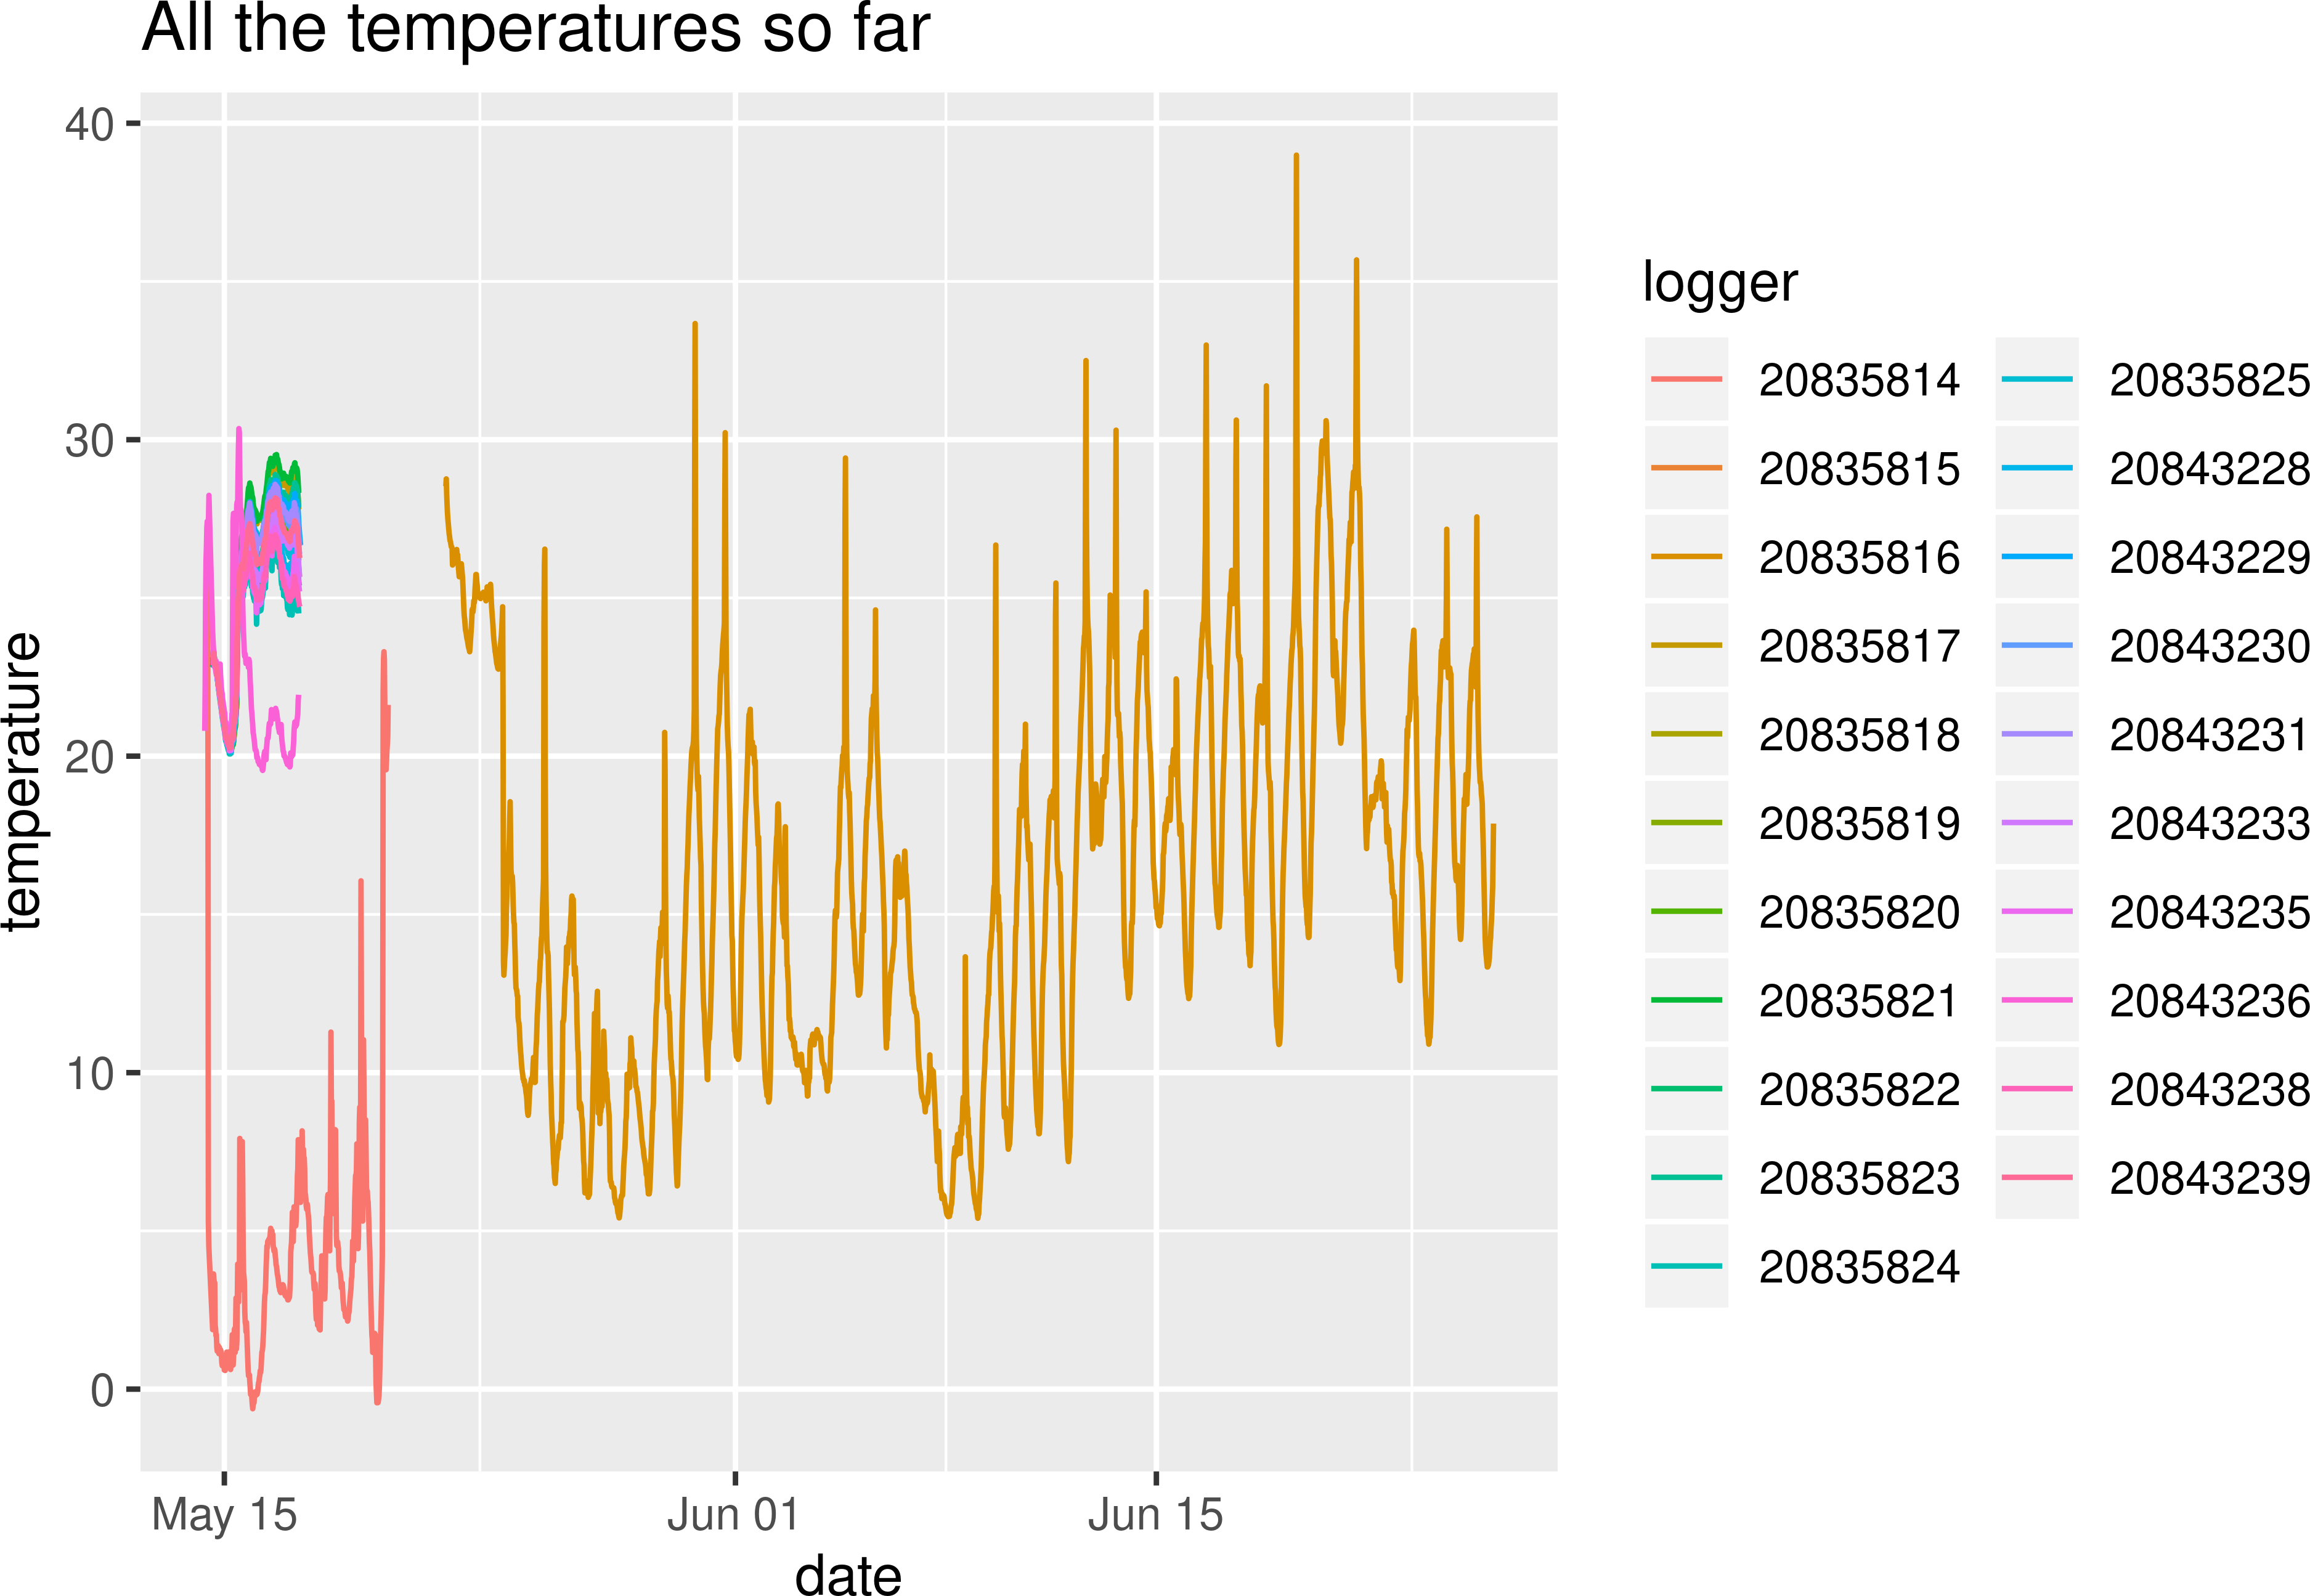
\includegraphics{figure/unnamed-chunk-12-1.png}

\begin{Shaded}
\begin{Highlighting}[]
\NormalTok{oneLogger <-}\StringTok{ }\NormalTok{combDat }\OperatorTok\StringTok{ }
\StringTok{  }\KeywordTok{filter}\NormalTok{(logger_id }\OperatorTok{==}\StringTok{ "20835815"}\NormalTok{) }\OperatorTok\StringTok{ }
\StringTok{  }\KeywordTok{select}\NormalTok{(}\DataTypeTok{Date =}\NormalTok{ date, }
\NormalTok{         logger_id,}
         \DataTypeTok{Temperature =}\NormalTok{ temperature,}
         \DataTypeTok{Relative_humidity =}\NormalTok{ rh,}
         \DataTypeTok{Dew_point =}\NormalTok{ dew) }\OperatorTok\StringTok{ }
\StringTok{  }\KeywordTok{pivot_longer}\NormalTok{(}\OperatorTok{-}\KeywordTok{c}\NormalTok{(Date, logger_id),}
               \DataTypeTok{names_to =} \StringTok{"Data_type"}\NormalTok{,}
               \DataTypeTok{values_to =} \StringTok{"Values"}\NormalTok{)}
  
\KeywordTok{ggplot}\NormalTok{(oneLogger) }\OperatorTok{+}
\StringTok{  }\KeywordTok{geom_line}\NormalTok{(}\KeywordTok{aes}\NormalTok{(}\DataTypeTok{x =}\NormalTok{ Date, }\DataTypeTok{y =}\NormalTok{ Values, }\DataTypeTok{color =}\NormalTok{ Data_type)) }\OperatorTok{+}
\StringTok{  }\KeywordTok{scale_color_nina}\NormalTok{() }\OperatorTok{+}
\StringTok{  }\KeywordTok{ggtitle}\NormalTok{(}\StringTok{"All the data from one logger"}\NormalTok{)}
\end{Highlighting}
\end{Shaded}

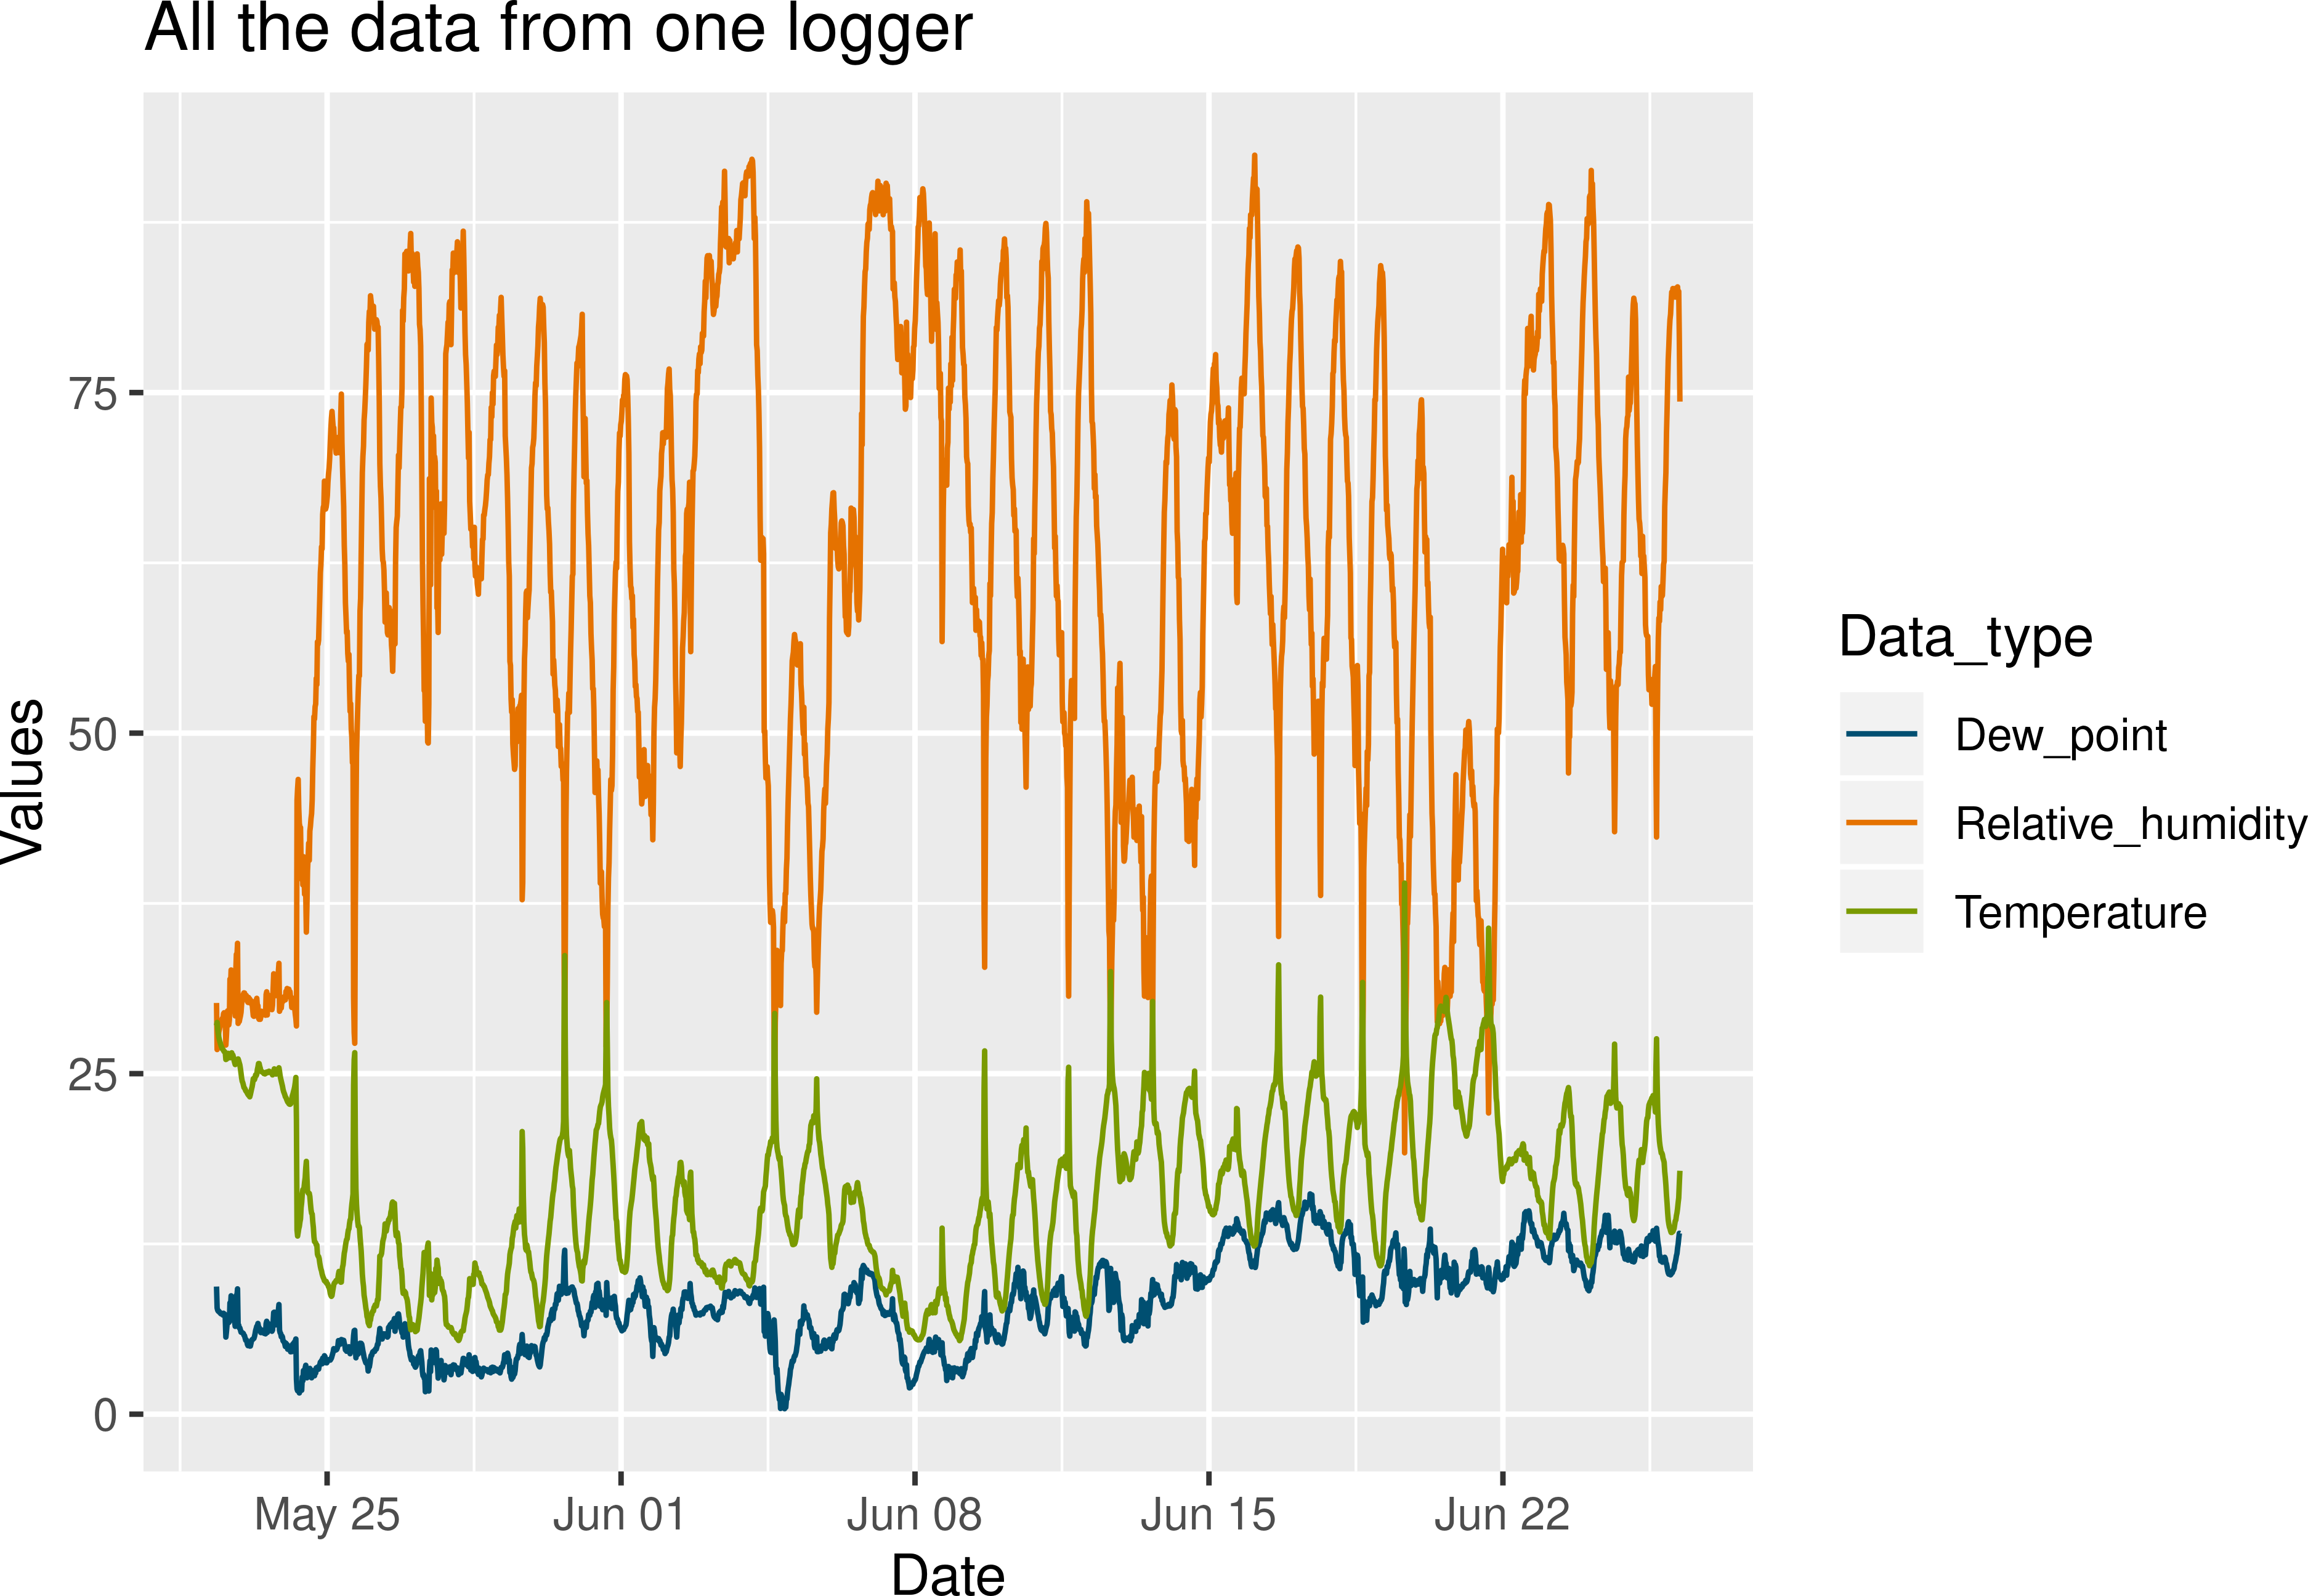
\includegraphics{figure/unnamed-chunk-13-1.png}

\hypertarget{combine-with-single-files-from-loggers-that-werent-synced}{%
\section{Combine with single files from loggers that weren't
synced}\label{combine-with-single-files-from-loggers-that-werent-synced}}

We had some troubles with the uploads from HoboConnect to Hobolink.com
from the CAT-phones. So the logger files from Oslo is provided
individually by email. Time to combine these as well. These have a
different data format than the export from hobolink. They also have some
extra columns at the end, which we can disregard.

\begin{Shaded}
\begin{Highlighting}[]
\NormalTok{formatMX2301File <-}\StringTok{ }\ControlFlowTok{function}\NormalTok{(inputFile)\{}
\NormalTok{raw <-}\StringTok{ }\KeywordTok{read_csv}\NormalTok{(}\DataTypeTok{file =}\NormalTok{ inputFile,}
                \DataTypeTok{col_types =} \KeywordTok{cols}\NormalTok{())}

\NormalTok{logger_id <-}\StringTok{ }\KeywordTok{gsub}\NormalTok{(}\StringTok{"(.*/)([0-9]*)( .*)"}\NormalTok{, }\StringTok{"}\CharTok{\textbackslash{}\textbackslash{}}\StringTok{2"}\NormalTok{, inputFile)}
  
\NormalTok{out <-}\StringTok{ }\NormalTok{raw }\OperatorTok\StringTok{ }
\StringTok{  }\KeywordTok{mutate}\NormalTok{(}\DataTypeTok{logger_id =}\NormalTok{ logger_id,}
         \DataTypeTok{date =} \KeywordTok{as.POSIXct}\NormalTok{(}\StringTok{`}\DataTypeTok{Date-Time (CET)}\StringTok{`}\NormalTok{, }\DataTypeTok{format =} \StringTok{"%m.%d.%Y %H.%M.%S"}\NormalTok{),}
         \DataTypeTok{temperature =} \KeywordTok{as.double}\NormalTok{(}\StringTok{`}\DataTypeTok{Ch: 1 - Temperature  °C (°C)}\StringTok{`}\NormalTok{),}
         \DataTypeTok{rh =} \KeywordTok{as.double}\NormalTok{(}\StringTok{`}\DataTypeTok{Ch: 2 - RH  % (%)}\StringTok{`}\NormalTok{),}
         \DataTypeTok{dew =} \KeywordTok{as.double}\NormalTok{(}\StringTok{`}\DataTypeTok{Dew Point  °C (°C)}\StringTok{`}\NormalTok{),}
         \DataTypeTok{logger_type =} \StringTok{"MX2301A"}\NormalTok{) }\OperatorTok\StringTok{ }
\StringTok{  }\KeywordTok{select}\NormalTok{(date,}
\NormalTok{         logger_type,}
\NormalTok{         logger_id,}
\NormalTok{         temperature,}
\NormalTok{         rh,}
\NormalTok{         dew)}

\KeywordTok{return}\NormalTok{(out)}

\NormalTok{\}}
\end{Highlighting}
\end{Shaded}

\begin{Shaded}
\begin{Highlighting}[]
\NormalTok{logger_}\DecValTok{20835817}\NormalTok{ <-}\StringTok{ }\KeywordTok{formatMX2301File}\NormalTok{(}\StringTok{"../rawData/20835817 2020-10-13 12_18_01 CET (Data CET).csv"}\NormalTok{)}
\end{Highlighting}
\end{Shaded}

\begin{verbatim}
## Warning: 10726 parsing failures.
## row col  expected     actual                                                         file
##   1  -- 8 columns 11 columns '../rawData/20835817 2020-10-13 12_18_01 CET (Data CET).csv'
##   2  -- 8 columns 11 columns '../rawData/20835817 2020-10-13 12_18_01 CET (Data CET).csv'
##   3  -- 8 columns 11 columns '../rawData/20835817 2020-10-13 12_18_01 CET (Data CET).csv'
##   4  -- 8 columns 11 columns '../rawData/20835817 2020-10-13 12_18_01 CET (Data CET).csv'
##   5  -- 8 columns 11 columns '../rawData/20835817 2020-10-13 12_18_01 CET (Data CET).csv'
## ... ... ......... .......... ............................................................
## See problems(...) for more details.
\end{verbatim}

\begin{Shaded}
\begin{Highlighting}[]
\NormalTok{logger_}\DecValTok{20835819}\NormalTok{ <-}\StringTok{ }\KeywordTok{formatMX2301File}\NormalTok{(}\StringTok{"../rawData/20835819 2020-10-14 14_33_12 CET (Data CET).csv"}\NormalTok{)}
\end{Highlighting}
\end{Shaded}

\begin{verbatim}
## Warning: 10803 parsing failures.
## row col  expected     actual                                                         file
##   1  -- 8 columns 11 columns '../rawData/20835819 2020-10-14 14_33_12 CET (Data CET).csv'
##   2  -- 8 columns 11 columns '../rawData/20835819 2020-10-14 14_33_12 CET (Data CET).csv'
##   3  -- 8 columns 11 columns '../rawData/20835819 2020-10-14 14_33_12 CET (Data CET).csv'
##   4  -- 8 columns 11 columns '../rawData/20835819 2020-10-14 14_33_12 CET (Data CET).csv'
##   5  -- 8 columns 11 columns '../rawData/20835819 2020-10-14 14_33_12 CET (Data CET).csv'
## ... ... ......... .......... ............................................................
## See problems(...) for more details.
\end{verbatim}

\begin{Shaded}
\begin{Highlighting}[]
\NormalTok{logger_}\DecValTok{20835820}\NormalTok{ <-}\StringTok{ }\KeywordTok{formatMX2301File}\NormalTok{(}\StringTok{"../rawData/20835820 2020-10-16 14_09_17 CET (Data CET).csv"}\NormalTok{)}
\end{Highlighting}
\end{Shaded}

\begin{verbatim}
## Warning: 10948 parsing failures.
## row col  expected     actual                                                         file
##   1  -- 8 columns 11 columns '../rawData/20835820 2020-10-16 14_09_17 CET (Data CET).csv'
##   2  -- 8 columns 11 columns '../rawData/20835820 2020-10-16 14_09_17 CET (Data CET).csv'
##   3  -- 8 columns 11 columns '../rawData/20835820 2020-10-16 14_09_17 CET (Data CET).csv'
##   4  -- 8 columns 11 columns '../rawData/20835820 2020-10-16 14_09_17 CET (Data CET).csv'
##   5  -- 8 columns 11 columns '../rawData/20835820 2020-10-16 14_09_17 CET (Data CET).csv'
## ... ... ......... .......... ............................................................
## See problems(...) for more details.
\end{verbatim}

\begin{Shaded}
\begin{Highlighting}[]
\NormalTok{logger_}\DecValTok{20835821}\NormalTok{ <-}\StringTok{ }\KeywordTok{formatMX2301File}\NormalTok{(}\StringTok{"../rawData/20835821 2020-10-15 15_49_08 CET (Data CET).csv"}\NormalTok{)}
\end{Highlighting}
\end{Shaded}

\begin{verbatim}
## Warning: 10880 parsing failures.
## row col  expected     actual                                                         file
##   1  -- 8 columns 11 columns '../rawData/20835821 2020-10-15 15_49_08 CET (Data CET).csv'
##   2  -- 8 columns 11 columns '../rawData/20835821 2020-10-15 15_49_08 CET (Data CET).csv'
##   3  -- 8 columns 11 columns '../rawData/20835821 2020-10-15 15_49_08 CET (Data CET).csv'
##   4  -- 8 columns 11 columns '../rawData/20835821 2020-10-15 15_49_08 CET (Data CET).csv'
##   5  -- 8 columns 11 columns '../rawData/20835821 2020-10-15 15_49_08 CET (Data CET).csv'
## ... ... ......... .......... ............................................................
## See problems(...) for more details.
\end{verbatim}

\begin{Shaded}
\begin{Highlighting}[]
\NormalTok{logger_}\DecValTok{20835823}\NormalTok{ <-}\StringTok{ }\KeywordTok{formatMX2301File}\NormalTok{(}\StringTok{"../rawData/20835823 2020-10-15 12_11_02 CET (Data CET).csv"}\NormalTok{)}
\end{Highlighting}
\end{Shaded}

\begin{verbatim}
## Warning: 10869 parsing failures.
## row col  expected     actual                                                         file
##   1  -- 8 columns 11 columns '../rawData/20835823 2020-10-15 12_11_02 CET (Data CET).csv'
##   2  -- 8 columns 11 columns '../rawData/20835823 2020-10-15 12_11_02 CET (Data CET).csv'
##   3  -- 8 columns 11 columns '../rawData/20835823 2020-10-15 12_11_02 CET (Data CET).csv'
##   4  -- 8 columns 11 columns '../rawData/20835823 2020-10-15 12_11_02 CET (Data CET).csv'
##   5  -- 8 columns 11 columns '../rawData/20835823 2020-10-15 12_11_02 CET (Data CET).csv'
## ... ... ......... .......... ............................................................
## See problems(...) for more details.
\end{verbatim}

\begin{Shaded}
\begin{Highlighting}[]
\NormalTok{logger_}\DecValTok{20843228}\NormalTok{ <-}\StringTok{ }\KeywordTok{formatMX2301File}\NormalTok{(}\StringTok{"../rawData/20843228 2020-10-14 11_43_58 CET (Data CET).csv"}\NormalTok{)}
\end{Highlighting}
\end{Shaded}

\begin{verbatim}
## Warning: 10794 parsing failures.
## row col  expected     actual                                                         file
##   1  -- 8 columns 11 columns '../rawData/20843228 2020-10-14 11_43_58 CET (Data CET).csv'
##   2  -- 8 columns 11 columns '../rawData/20843228 2020-10-14 11_43_58 CET (Data CET).csv'
##   3  -- 8 columns 11 columns '../rawData/20843228 2020-10-14 11_43_58 CET (Data CET).csv'
##   4  -- 8 columns 11 columns '../rawData/20843228 2020-10-14 11_43_58 CET (Data CET).csv'
##   5  -- 8 columns 11 columns '../rawData/20843228 2020-10-14 11_43_58 CET (Data CET).csv'
## ... ... ......... .......... ............................................................
## See problems(...) for more details.
\end{verbatim}

\begin{Shaded}
\begin{Highlighting}[]
\NormalTok{logger_}\DecValTok{20843229}\NormalTok{ <-}\StringTok{ }\KeywordTok{formatMX2301File}\NormalTok{(}\StringTok{"../rawData/20843229 2020-10-16 09_59_17 CET (Data CET).csv"}\NormalTok{)}
\end{Highlighting}
\end{Shaded}

\begin{verbatim}
## Warning: 10930 parsing failures.
## row col  expected     actual                                                         file
##   1  -- 8 columns 11 columns '../rawData/20843229 2020-10-16 09_59_17 CET (Data CET).csv'
##   2  -- 8 columns 11 columns '../rawData/20843229 2020-10-16 09_59_17 CET (Data CET).csv'
##   3  -- 8 columns 11 columns '../rawData/20843229 2020-10-16 09_59_17 CET (Data CET).csv'
##   4  -- 8 columns 11 columns '../rawData/20843229 2020-10-16 09_59_17 CET (Data CET).csv'
##   5  -- 8 columns 11 columns '../rawData/20843229 2020-10-16 09_59_17 CET (Data CET).csv'
## ... ... ......... .......... ............................................................
## See problems(...) for more details.
\end{verbatim}

\begin{Shaded}
\begin{Highlighting}[]
\NormalTok{logger_}\DecValTok{20843233}\NormalTok{ <-}\StringTok{ }\KeywordTok{formatMX2301File}\NormalTok{(}\StringTok{"../rawData/20843233 2020-10-14 16_25_22 CET (Data CET).csv"}\NormalTok{)}
\end{Highlighting}
\end{Shaded}

\begin{verbatim}
## Warning: 10808 parsing failures.
## row col  expected     actual                                                         file
##   1  -- 8 columns 11 columns '../rawData/20843233 2020-10-14 16_25_22 CET (Data CET).csv'
##   2  -- 8 columns 11 columns '../rawData/20843233 2020-10-14 16_25_22 CET (Data CET).csv'
##   3  -- 8 columns 11 columns '../rawData/20843233 2020-10-14 16_25_22 CET (Data CET).csv'
##   4  -- 8 columns 11 columns '../rawData/20843233 2020-10-14 16_25_22 CET (Data CET).csv'
##   5  -- 8 columns 11 columns '../rawData/20843233 2020-10-14 16_25_22 CET (Data CET).csv'
## ... ... ......... .......... ............................................................
## See problems(...) for more details.
\end{verbatim}

\begin{Shaded}
\begin{Highlighting}[]
\NormalTok{logger_}\DecValTok{20843238}\NormalTok{ <-}\StringTok{ }\KeywordTok{formatMX2301File}\NormalTok{(}\StringTok{"../rawData/20843238 2020-10-16 16_52_35 CET (Data CET).csv"}\NormalTok{)}
\end{Highlighting}
\end{Shaded}

\begin{verbatim}
## Warning: 10953 parsing failures.
## row col  expected     actual                                                         file
##   1  -- 8 columns 11 columns '../rawData/20843238 2020-10-16 16_52_35 CET (Data CET).csv'
##   2  -- 8 columns 11 columns '../rawData/20843238 2020-10-16 16_52_35 CET (Data CET).csv'
##   3  -- 8 columns 11 columns '../rawData/20843238 2020-10-16 16_52_35 CET (Data CET).csv'
##   4  -- 8 columns 11 columns '../rawData/20843238 2020-10-16 16_52_35 CET (Data CET).csv'
##   5  -- 8 columns 11 columns '../rawData/20843238 2020-10-16 16_52_35 CET (Data CET).csv'
## ... ... ......... .......... ............................................................
## See problems(...) for more details.
\end{verbatim}

Combine these files to the other ones.

\begin{Shaded}
\begin{Highlighting}[]
\NormalTok{allMX2301 <-}\StringTok{ }\NormalTok{combDat2 }\OperatorTok\StringTok{ }
\StringTok{  }\KeywordTok{rbind}\NormalTok{(logger_}\DecValTok{20835817}\NormalTok{) }\OperatorTok\StringTok{ }
\StringTok{  }\KeywordTok{rbind}\NormalTok{(logger_}\DecValTok{20835819}\NormalTok{) }\OperatorTok\StringTok{ }
\StringTok{  }\KeywordTok{rbind}\NormalTok{(logger_}\DecValTok{20835820}\NormalTok{) }\OperatorTok\StringTok{ }
\StringTok{  }\KeywordTok{rbind}\NormalTok{(logger_}\DecValTok{20835821}\NormalTok{) }\OperatorTok\StringTok{ }
\StringTok{  }\KeywordTok{rbind}\NormalTok{(logger_}\DecValTok{20835823}\NormalTok{) }\OperatorTok\StringTok{ }
\StringTok{  }\KeywordTok{rbind}\NormalTok{(logger_}\DecValTok{20843228}\NormalTok{) }\OperatorTok\StringTok{ }
\StringTok{  }\KeywordTok{rbind}\NormalTok{(logger_}\DecValTok{20843229}\NormalTok{) }\OperatorTok\StringTok{ }
\StringTok{  }\KeywordTok{rbind}\NormalTok{(logger_}\DecValTok{20843233}\NormalTok{) }\OperatorTok\StringTok{ }
\StringTok{  }\KeywordTok{rbind}\NormalTok{(logger_}\DecValTok{20843238}\NormalTok{) }
\end{Highlighting}
\end{Shaded}

\hypertarget{handle-the-mx2201-loggers}{%
\section{Handle the MX2201 loggers}\label{handle-the-mx2201-loggers}}

These are temperature and light loggers that where also placed at some
locations (that also had sound loggers). They have slightly different
format, so we adapt the function to handle these.

\begin{Shaded}
\begin{Highlighting}[]
\NormalTok{longerHobo2202 <-}\StringTok{ }\ControlFlowTok{function}\NormalTok{(inputFile)\{}
\NormalTok{rawDat <-}\StringTok{ }\KeywordTok{read_csv}\NormalTok{(inputFile,}
                   \DataTypeTok{guess_max =} \DecValTok{10000}\NormalTok{,}
                   \DataTypeTok{col_types =} \KeywordTok{cols}\NormalTok{())}

\NormalTok{  dat <-}\StringTok{ }\NormalTok{rawDat }\OperatorTok\StringTok{  }
\StringTok{    }\KeywordTok{select}\NormalTok{(}\OperatorTok{-}\StringTok{"Line#"}\NormalTok{) }\OperatorTok\StringTok{ }
\StringTok{    }\KeywordTok{mutate}\NormalTok{(}\DataTypeTok{date =} \KeywordTok{as.POSIXct}\NormalTok{(Date, }\DataTypeTok{format =} \StringTok{"%m/%d/%y %H:%M:%S"}\NormalTok{)) }\OperatorTok\StringTok{ }
\StringTok{    }\KeywordTok{mutate_if}\NormalTok{(is_character, as.double) }\OperatorTok\StringTok{ }
\StringTok{    }\KeywordTok{select}\NormalTok{(}\OperatorTok{-}\NormalTok{Date)}


   
\NormalTok{  temp <-}\StringTok{ }\NormalTok{dat }\OperatorTok\StringTok{ }
\StringTok{    }\KeywordTok{pivot_longer}\NormalTok{(}\DataTypeTok{cols =} \KeywordTok{starts_with}\NormalTok{(}\StringTok{"Temperature"}\NormalTok{),}
               \DataTypeTok{names_to =} \StringTok{"logger_id"}\NormalTok{,}
               \DataTypeTok{values_to =} \StringTok{"temperature"}\NormalTok{) }\OperatorTok\StringTok{ }
\StringTok{    }\KeywordTok{select}\NormalTok{(date,}
\NormalTok{         logger_id,}
\NormalTok{         temperature) }\OperatorTok\StringTok{ }
\StringTok{    }\KeywordTok{filter}\NormalTok{(}\OperatorTok{!}\KeywordTok{is.na}\NormalTok{(temperature))}

\NormalTok{  light <-}\StringTok{ }\NormalTok{dat }\OperatorTok\StringTok{ }
\StringTok{    }\KeywordTok{pivot_longer}\NormalTok{(}\DataTypeTok{cols =} \KeywordTok{starts_with}\NormalTok{(}\StringTok{"Light"}\NormalTok{),}
                 \DataTypeTok{names_to =} \StringTok{"logger_id"}\NormalTok{,}
                 \DataTypeTok{values_to =} \StringTok{"light"}\NormalTok{) }\OperatorTok\StringTok{ }
\StringTok{    }\KeywordTok{select}\NormalTok{(date,}
\NormalTok{           logger_id,}
\NormalTok{           light)}\OperatorTok\StringTok{ }
\StringTok{    }\KeywordTok{filter}\NormalTok{(}\OperatorTok{!}\KeywordTok{is.na}\NormalTok{(light))}
  
  
  
\NormalTok{  temp <-}\StringTok{ }\NormalTok{temp }\OperatorTok\StringTok{ }
\StringTok{    }\KeywordTok{mutate}\NormalTok{(}\DataTypeTok{logger_id =} \KeywordTok{str_extract}\NormalTok{(logger_id,}
                              \StringTok{"[^, ]+$"}\NormalTok{))}
\NormalTok{  light <-}\StringTok{ }\NormalTok{light }\OperatorTok\StringTok{ }
\StringTok{    }\KeywordTok{mutate}\NormalTok{(}\DataTypeTok{logger_id =} \KeywordTok{str_extract}\NormalTok{(logger_id,}
                                \StringTok{"[^, ]+$"}\NormalTok{))}

  \ControlFlowTok{if}\NormalTok{(}\OperatorTok{!}\KeywordTok{all}\NormalTok{(temp}\OperatorTok{$}\NormalTok{date }\OperatorTok{==}\StringTok{ }\NormalTok{light}\OperatorTok{$}\NormalTok{date)) }\KeywordTok{stop}\NormalTok{(}\StringTok{"Tables datetimes doesn't match"}\NormalTok{)}
  
\NormalTok{  combDat <-}\StringTok{ }\NormalTok{temp }\OperatorTok\StringTok{ }
\StringTok{  }\KeywordTok{full_join}\NormalTok{(light,}
             \DataTypeTok{by =} \KeywordTok{c}\NormalTok{(}\StringTok{"date"}\NormalTok{ =}\StringTok{ "date"}\NormalTok{,}
                    \StringTok{"logger_id"}\NormalTok{ =}\StringTok{ "logger_id"}\NormalTok{)) }\OperatorTok\StringTok{ }
\StringTok{  }\KeywordTok{arrange}\NormalTok{(logger_id,}
\NormalTok{          date) }\OperatorTok\StringTok{ }
\StringTok{    }\KeywordTok{mutate}\NormalTok{(}\DataTypeTok{logger_type =} \StringTok{"MX2202"}\NormalTok{) }\OperatorTok\StringTok{ }
\StringTok{    }\KeywordTok{select}\NormalTok{(date, }
\NormalTok{           logger_type,}
\NormalTok{           logger_id,}
\NormalTok{           temperature,}
\NormalTok{           light)}
  
  \KeywordTok{return}\NormalTok{(combDat)}
\NormalTok{\}}
\end{Highlighting}
\end{Shaded}

\begin{Shaded}
\begin{Highlighting}[]
\NormalTok{allMX2202 <-}\StringTok{ }\KeywordTok{longerHobo2202}\NormalTok{(}\DataTypeTok{inputFile =} \StringTok{"../rawData/Insect_MX2202_temp_light_2020_10_27_13_02_59_UTC_1.csv"}\NormalTok{)}
\end{Highlighting}
\end{Shaded}

\begin{verbatim}
## Warning in mask$eval_all_mutate(dots[[i]]): NAs introduced by coercion
\end{verbatim}

\hypertarget{write-the-data-to-the-database}{%
\section{Write the data to the
database}\label{write-the-data-to-the-database}}

In the database, we combine the logger types into one table, and make it
even longer. I.e. we combine all values in one column. (Many ways to do
this).

\begin{Shaded}
\begin{Highlighting}[]
\NormalTok{allMX2301Long <-}\StringTok{ }\NormalTok{allMX2301 }\OperatorTok\StringTok{ }
\StringTok{  }\KeywordTok{pivot_longer}\NormalTok{(}\DataTypeTok{cols =} \KeywordTok{c}\NormalTok{(}\StringTok{"temperature"}\NormalTok{, }\StringTok{"rh"}\NormalTok{, }\StringTok{"dew"}\NormalTok{),}
               \DataTypeTok{names_to =} \StringTok{"data_type"}\NormalTok{)}

\NormalTok{allMX2202Long <-}\StringTok{ }\NormalTok{allMX2202 }\OperatorTok\StringTok{ }
\StringTok{  }\KeywordTok{pivot_longer}\NormalTok{(}\DataTypeTok{cols =} \KeywordTok{c}\NormalTok{(}\StringTok{"temperature"}\NormalTok{, }\StringTok{"light"}\NormalTok{),}
               \DataTypeTok{names_to =} \StringTok{"data_type"}\NormalTok{)}

\NormalTok{allLoggersLong <-}\StringTok{ }\NormalTok{allMX2301Long }\OperatorTok\StringTok{ }
\StringTok{  }\KeywordTok{rbind}\NormalTok{(allMX2202Long)}
\end{Highlighting}
\end{Shaded}

\hypertarget{make-the-database-table}{%
\subsection{Make the database table}\label{make-the-database-table}}

\begin{Shaded}
\begin{Highlighting}[]
\NormalTok{createLoggerSchemaQ <-}\StringTok{ "}
\StringTok{CREATE SCHEMA IF NOT EXISTS loggers;}
\StringTok{"}

\NormalTok{createLoggerTableQ <-}\StringTok{ "}
\StringTok{CREATE TABLE IF NOT EXISTS loggers.logger_data (}
\StringTok{--id uuid NOT NULL DEFAULT gen_random_uuid(),}
\StringTok{id serial NOT NULL,}
\StringTok{date timestamptz NOT NULL,}
\StringTok{logger_type text NOT NULL,}
\StringTok{logger_id integer NOT NULL,}
\StringTok{data_type text NOT NULL,}
\StringTok{value double precision}
\StringTok{);}

\StringTok{"}

\KeywordTok{dbSendQuery}\NormalTok{(con, createLoggerSchemaQ)}
\KeywordTok{dbSendQuery}\NormalTok{(con, createLoggerTableQ)}

\KeywordTok{dbSendQuery}\NormalTok{(con,}
            \StringTok{"CREATE INDEX ON loggers.logger_data USING BTREE(date);"}\NormalTok{)}

\KeywordTok{dbSendQuery}\NormalTok{(con,}
            \StringTok{"CREATE INDEX ON loggers.logger_data USING BTREE(logger_type);"}\NormalTok{)}

\KeywordTok{dbSendQuery}\NormalTok{(con,}
            \StringTok{"CREATE INDEX ON loggers.logger_data USING BTREE(logger_id);"}\NormalTok{)}

\KeywordTok{dbSendQuery}\NormalTok{(con,}
            \StringTok{"CREATE INDEX ON loggers.logger_data USING BTREE(data_type);"}\NormalTok{)}
\end{Highlighting}
\end{Shaded}

\begin{Shaded}
\begin{Highlighting}[]
\KeywordTok{dbWriteTable}\NormalTok{(con, }
             \DataTypeTok{name =} \KeywordTok{Id}\NormalTok{(}\DataTypeTok{schema =} \StringTok{"loggers"}\NormalTok{, }\DataTypeTok{table =} \StringTok{"logger_data"}\NormalTok{),}
             \DataTypeTok{value =}\NormalTok{ allLoggersLong,}
             \DataTypeTok{append =}\NormalTok{ T}
\NormalTok{             )}
\end{Highlighting}
\end{Shaded}

Read in logger deployments

\begin{Shaded}
\begin{Highlighting}[]
\NormalTok{logger_deployments <-}\StringTok{ }\KeywordTok{read_delim}\NormalTok{(}\StringTok{"../../../Data/klimalogger/logger_deployments_2020.csv"}\NormalTok{,}
                               \DataTypeTok{delim =} \StringTok{";"}\NormalTok{)}
\end{Highlighting}
\end{Shaded}

\begin{verbatim}
## Parsed with column specification:
## cols(
##   logger_id = col_double(),
##   logger_type = col_character(),
##   year = col_double(),
##   location = col_character()
## )
\end{verbatim}

\begin{Shaded}
\begin{Highlighting}[]
\NormalTok{createLoggerDeploymentsQ <-}\StringTok{ "}
\StringTok{CREATE TABLE IF NOT EXISTS loggers.logger_deployments (}
\StringTok{--id uuid NOT NULL DEFAULT gen_random_uuid(),}
\StringTok{id serial PRIMARY KEY,}
\StringTok{logger_id integer NOT NULL,}
\StringTok{logger_type text NOT NULL,}
\StringTok{year integer NOT NULL,}
\StringTok{location text NOT NULL}
\StringTok{);}
\StringTok{"}
\KeywordTok{dbSendQuery}\NormalTok{(con, createLoggerDeploymentsQ)}

\KeywordTok{dbSendQuery}\NormalTok{(con,}
            \StringTok{"CREATE INDEX ON loggers.logger_deployments USING BTREE(logger_id);"}\NormalTok{)}

\KeywordTok{dbSendQuery}\NormalTok{(con,}
            \StringTok{"CREATE INDEX ON loggers.logger_deployments USING BTREE(logger_type);"}\NormalTok{)}

\KeywordTok{dbSendQuery}\NormalTok{(con,}
            \StringTok{"CREATE INDEX ON loggers.logger_deployments USING BTREE(year);"}\NormalTok{)}

\KeywordTok{dbSendQuery}\NormalTok{(con,}
            \StringTok{"CREATE INDEX ON loggers.logger_deployments USING BTREE(location);"}\NormalTok{)}
\end{Highlighting}
\end{Shaded}

\begin{Shaded}
\begin{Highlighting}[]
\KeywordTok{dbWriteTable}\NormalTok{(con,}
             \DataTypeTok{name =} \KeywordTok{Id}\NormalTok{(}\DataTypeTok{schema =} \StringTok{"loggers"}\NormalTok{, }\DataTypeTok{table =} \StringTok{"logger_deployments"}\NormalTok{),}
             \DataTypeTok{value =}\NormalTok{ logger_deployments,}
             \DataTypeTok{append =}\NormalTok{ T}
\NormalTok{             )}
\end{Highlighting}
\end{Shaded}

\hypertarget{write-the-data-as-csv}{%
\section{Write the data as CSV}\label{write-the-data-as-csv}}

We also write the data as csv files, if we don't want to use the
database.

\begin{Shaded}
\begin{Highlighting}[]
\KeywordTok{write_csv}\NormalTok{(allLoggersLong, }\DataTypeTok{path =} \StringTok{"../out/insectLogger_data_2020.csv"}\NormalTok{)}
\KeywordTok{write_csv}\NormalTok{(logger_deployments, }\DataTypeTok{path =} \StringTok{"../out/insect_logger_deployments.csv"}\NormalTok{)}
\end{Highlighting}
\end{Shaded}


\end{document}
